%! TeX program = lualatex
\documentclass[twoside, a4paper, 12pt]{book}

\title{Teoria kategorii}
\author{\color{subtext1}Weronika Jakimowicz}
\date{Lato 2024/25}

\usepackage[dates, pl]{../../../template}

\fancyfoot[CE, CO]{}
\fancyfoot[LE, RO]{\color{overlay2}\thepage}

\fancyhead[RE, LO]{$ \quad $\color{subtext1}koneser kategorii $ \quad $}
\fancyhead[LE, RO]{$ \quad $\color{green!40!subtext2}\bfseries\htitle $ \quad $}

\fancypagestyle{plain}{%
  \fancyhf{}%
  \fancyfoot[CE, CO]{}
  \fancyfoot[LE, RO]{\color{overlay2}\thepage}

  \fancyhead[RE, LO]{$ \quad $\color{subtext1}abstrakcyjne smaczki $ \quad $}
  \fancyhead[LE, RO]{$ \quad $\color{green!40!subtext2}\bfseries\htitle $ \quad $}
}

\begin{document}
\frontmatter 
\maketitle
\thispagestyle{empty}
\setcounter{page}{0}

\tableofcontents
\mainmatter

\pagestyle{fancy}

\chapter{Początek końca}

Głównym bohaterem będzie krzywizna.

\section{25.02.2025}{Rozgrzewka}

\subsection{Krzywe na płaszczyźnie}

Jakościowo opisać krzywiznę krzywej na płaszczyźnie jest łatwo. Chcemy to zrobić bardziej matematycznie. 

Patrzymy na okrąg na płaszczyźnie, który powinien mieć taką samą krzywiznę w każdym punkcie. Dodatkowo, im większy okrąg tym mniejsza krzywizna.
\begin{center}
  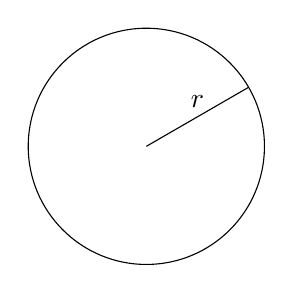
\begin{tikzpicture}
    \draw (0,0) circle (1.5);
    \draw (0,0)-- node[above] {$r$} (30:1.5);
  \end{tikzpicture}
\end{center}
Dla okręgu jak wyżej definiujemy krzywiznę
$$\kappa=\frac{1}{r}$$

Niech $\gamma$ będzie różniczkowalną krzywą gładką o niezerowej pochodnej. Wyobraźmy sobie okrąg, który podróżuje po krzywej $\gamma$ z prędkością $\gamma'(t)$ zależną od punktu na krzywej
\begin{center}
  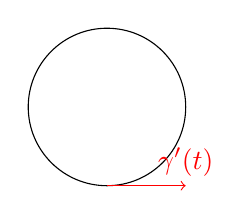
\begin{tikzpicture}
    \draw (0,0) circle (1);
    % \draw (-1.5, -1)--(.5, -1) to[out=0, in=-90] (.7, 0) to[out=90, in=-90] (.3, 1);
    \draw[red, ->] (0, -1) to (1, -1) node[above] {$\gamma'(t)$};
  \end{tikzpicture}
\end{center}
Na tym okręgu działa pewna siła odśrodkowa - to będzie nasza krzywizna.

\begin{definition}{}{}
  Krzywa regularna to gładkie odwzorowanie
  $$\gamma:(a,b)\to\R^2$$
  której pochodna jest niezerowa w każdym punkcie $\gamma'(t)\neq 0$.
\end{definition}

\begin{lemma}{o parametryzacji łukowej}{}
  Jeżeli $\gamma:(a,b)\to\R^2$ jest krzywą regularną, to istnieje gładka reparametryzacja $s:(a,b)\to(0,l)$ taka, że $\gamma\circ s^{-1}$ jest krzywą o prędkości $1$. To znaczy, że 
  $$|(\gamma\circ s^{-1})'(d)|=1$$
  dla każdego $d\in(0,l)$.
\end{lemma}

\begin{proof}
  Zdefiniujmy $s$ 
  $$s(t)=\int_a^t|\gamma'(u)|du.$$
  Wtedy przeciwobraz krzywej $s$ w punkcie $u$ to droga, którą przebyliśmy od początku do teraz po krzywej $\gamma$:
  $$\int_a^{a+d}|(\gamma\circ s^{-1})'(u)|du=d$$
\end{proof}

\begin{example}
  Policzymy przyśpieszenie na okręgu. Wzór na okrąg to krzywa
  $$\gamma(t)=(r\cos t, r\sin t),\quad t\in[0,2\pi],$$
  więc nie jest to parametryzacja łukowa (długość łuku). Prosta zmiana daje nam
  $$\gamma(t)=(r\cos \frac{t}{r}, r\sin \frac{t}{r}),\quad t\in[0,2\pi r],$$
  którego pochodna to 
  $$\gamma'(t)=(-\sin\frac{t}{r}, \cos\frac{t}{r})$$
  wektor długości $1$.

  Druga pochodna $\gamma$, czyli siła dośrodkowa, to
  $$\gamma''(t)=(-\frac{1}{r}\cos\frac{t}{r}, -\frac{1}{r}\sin\frac{t}{s}),$$
  której wartość
  $$|\gamma''(t)|=\frac{1}{r}$$
  to faktycznie krzywizna okręgu.
\end{example}

\begin{lemma}{}{}
  Jeśli $\gamma$ jest sparametryzowane długością łuku, to $\gamma''(s)$ jest prostopadła do $\gamma'(s)$.
\end{lemma}

\begin{proof}
  Długość krzywej sparametryzowanej długością łuku
  $$\langle \gamma'(s), \gamma'(s)\rangle=1$$
  jest funkcją stałą. Jeśli więc zróżniczkujemy ją względem $s$, to dostajemy
  $$0=\frac{d}{ds}\langle \gamma'(s), \gamma'(s)\rangle=2\langle\gamma''(s),\gamma'(s)\rangle $$
\end{proof}

\begin{definition}{}{}
  Niech $\gamma$ będzie krzywą sparametryzowaną długością łuku. Niech $N(t)$ będzie wektorem jednostkowym ortogonalnym do $\gamma'(t)$ i takim, że 
  $$(\gamma'(t), N(t))$$
  jest dodatnio zorientowaną bazą $\R^2$:
  \begin{center}
    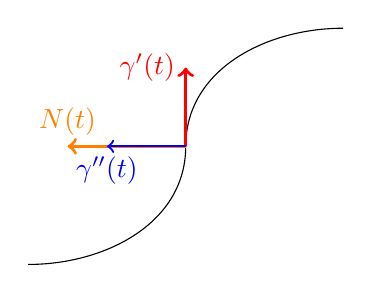
\begin{tikzpicture}
      \draw (-1,0) to[out=0, in=-90] (1, 1.5) to[out=90, in=180] (3, 3);
      \draw[red, very thick, ->] (1, 1.5) -- (1, 2.5) node[left] {$\gamma'(t)$};
      \draw[orange, very thick, ->] (1, 1.5)--(-.5, 1.5) node[above] {$N(t)$};
      \draw[blue, thick, ->] (1, 1.5)--(0, 1.5) node[below] {$\gamma''(t)$};
    \end{tikzpicture}
  \end{center}
  Krzywizna $\kappa_\gamma(t)$ (znakowana) w $t$ jest definiowana równaniem
  $$\gamma''(t)=\kappa_\gamma(t)N(t)$$
\end{definition}

\begin{example}
  Rozważamy parabolę, czyli krzywą daną jako
  $$\gamma(t)=(t, t^2).$$
  Naszym celem jest policzenie krzywizny w punkcie $t=0$. Wzór wyżej nie jest parametryzacja długością łuku. Liczymy więc obie pochodne:
  $$\gamma'(t)=(1, 2t)$$
  $$\gamma''(t)=(0, 2).$$
  Zauważamy, że druga pochodna nie jest prostopadła do prędkości, co zgadza się z intuicją, bo punkt podróżujący po paraboli coraz szybciej leci w górę. Liczymy nową parametryzację:
  $$s(t)=\int_0^t\sqrt{1+4u^2}du,$$
  której nie da się w łatwy sposób scałkować.
  $$\frac{ds}{dt}|_{t=0}=1$$
  z różniczkowania funkcji odwrotnej
  $$\frac{dt}{ds}|_{s=0}=\frac{1}{\frac{ds}{dt}}|_{t=0}=1$$
  Krzywizna to będzie 
  $$\frac{d}{ds}(\gamma\circ s^{-1})(s) =\frac{d}{ds}\gamma(t(s))=\frac{d\gamma}{dt}(t(s))\cdot\frac{dt}{ds}(s)$$
  $$\frac{d^2}{ds^2}\gamma(t(s))=\frac{d^2\gamma}{dt^2}\cdot\left(\frac{dt}{ds}\right)^2+\frac{d\gamma}{dt}\cdot\frac{d^2t}{ds^2}=(0,2)\cdot 1+(1,0)\frac{d^2t}{ds^2}$$
  i $\frac{d^2t}{ds^2}$ nie da się łatwo policzyć, więc korzystamy z faktu, że $(1,0)\frac{d^2t}{ds^2}$ jest prostopadłe do $\gamma'(0)=(1,0)$, jeśli $\gamma'$ jest sprametryzowane długością łuku, ale tutaj nie musimy uważać, bo pierwsza pochodna jest taka sama z dokładnością do mnożenia przez stałą bez względu na jej parametryzację. Stąd wiemy, że 
  $$\frac{d^2t}{ds^2}=0,$$
  bo iloczyn skalarny jest temu równy (z dokładnością do stałej).
\end{example}

\begin{lemma}{równania Freneta}{}
  Niech $\gamma$ będzie sparametryzowana długością łuku i niech $(T(s), N(s))$ będzie bazą ortonormalną dodatnio zorientowaną, gdzie $T(s)=\gamma'(s)$. Wtedy:
    $$T'=\kappa\cdot N$$
  $$N'=-\kappa T$$
\end{lemma}

\begin{proof}
  Pierwsze równanie to definicja krzywizny. W drugim równaniu trzeba zróżniczkować $N$.
  $$0=\frac{d}{ds}\langle N, N\rangle=2\langle N',N\rangle,$$
  czyli $N'=\alpha T$, gdzie 
  $$\alpha=\langle N', T\rangle=\langle N, T\rangle '-\langle N, T'\rangle$$
\end{proof}

\begin{theorem}{podstawowe twierdzenie teorii krzywych}{}
  Dla dowolnych $(x_0, y_0)\in \R^2$, jednostkowego wektora $v\in\R^2$ i gładkiej funkcji $\kappa:[0,b]\to \R^2$ istnieje dokładnie jedna krzywa $\gamma:[0,b]\to\R$ sparametryzowana długością łuku taka, że $\gamma(0)=(x_0, y_0)$, $\gamma'(0)=v$, $\kappa_\gamma=\kappa$.
\end{theorem}

\begin{proof}
  Niech $T=(T_1, T_2)$ i $T(0)=v$ i $N=(-T_2, T_1)$ będzie ramką Freneta. Wtedy
  $$\begin{pmatrix}T_1'\\T_2'\end{pmatrix}=\begin{pmatrix}-\kappa T_2\\\kappa T_1\end{pmatrix}=\begin{pmatrix}0 & -\kappa\\ \kappa & 0 \end{pmatrix}\begin{pmatrix}T_1\\T_2\end{pmatrix}$$
  jest jedynym rozwiązaniem 
  $$\gamma(s)=\int_0^sT(u)dy+(x_0, y_0).$$
  Wiemy, że $|T|=1$, bo 
  $$\frac{d}{ds}|T|^2=\frac{d}{ds}\langle T,T\rangle=2\langle T',T\rangle=0$$
\end{proof}

\begin{definition}{}{}
  Niech krzywa $\gamma$ będzie sparametryzowana długością łuku i niech $\eta$ będzie okręgiem sparametryzowanym długością łuku stycznym do $\gamma$ (wektory prędkości się pokrywają) w punkcie $\gamma(t_0)$. Wtedy $\neta$ jest \buff{okręgiem ściśle stycznym}, jeżeli $\eta''(t_0)=\gamma''(t_0)$.
\end{definition}

\begin{definition}{}{}
  \buff{Ewolutą krzywej} $\gamma$ nazywamy krzywą utworzoną ze środków okręgów ściśle do niej stycznych.
  $$c=\gamma+\frac{1}{\kappa}N$$
\end{definition}

W punktach przegięcia albo ignorujemy je i wymagamy, aby $\gamma''(t)\neq0$, albo mówimy, że w punkcie przegięcia okrąg ściśle styczny to prosta.

\begin{fact}{}{}
  Niech $\gamma$ będzie krzywą sparametryzowaną długością łuku taką, że $\kappa'(t)\neq 0$, to okręgi ściśle styczne są parami rozłącznew otoczeniu $t$.
\end{fact}

\begin{proof}
  Niech $c$ będzie ewolutą krzywej $\gamma$. Weźmy dwa punkty $t_1$ i $t_2$ w otoczeniu punktu $t$ z twierdzenia. Naszym celem będzie pokazanie, że długość drogi $c(t_1)$ a $c(t_2)$ jest nie większa niż różnica promieni:
  $$\int_{t_0}^{t_1}|c'(u)|du=\left|\frac{1}{R(t_0)}-\frac{1}{R(t_1)}\right|,$$
  gdzie $R(t_i)$ to promień okręgu ściśle stycznego do $\gamma$ w punkcie $t_i$.
  $$c'=\gamma'+\frac{1}{\kappa}N'+\left(\frac{1}{\kappa}\right)'N=T+\frac{1}{\kappa}(-\kappa T)+\left(\frac{1}{\kappa}\right)'N,$$
  czyli
  $$\int_{t_0}^{t_1}|c'(u)|du=\int_{t_0}^{t_1}\left|\left(\frac{1}{\kappa}\right)'\right| du=\left|\frac{1}{R(t_0)}-\frac{1}{R(t_1)}\right|.$$
\end{proof}




  
\end{document}
